\documentclass[12pt]{article}
\usepackage[left=1cm, right=1cm, top=2cm,bottom=1.5cm]{geometry} 

\usepackage[parfill]{parskip}
\usepackage[utf8]{inputenc}
\usepackage[T2A]{fontenc}
\usepackage[russian]{babel}
\usepackage{enumitem}
\usepackage[normalem]{ulem}
\usepackage{amsfonts, amsmath, amsthm, amssymb, mathtools}

\usepackage{fancyhdr}
\pagestyle{fancy}
\renewcommand{\headrulewidth}{1.5pt}
\renewcommand{\footrulewidth}{1pt}

\usepackage{graphicx}
\usepackage[figurename=Рис.]{caption}
\usepackage{subcaption}
\usepackage{float}

%%Наименование папки откуда забирать изображения
\graphicspath{ {./images/} }

%%Изменение формата для ввода доказательства
\renewcommand{\proofname}{$\square$  \nopunct}
\renewcommand\qedsymbol{$\blacksquare$}

\addto\captionsrussian{%
	\renewcommand{\proofname}{$\square$ \nopunct}%
}
%% Римские цифры
\newcommand{\RN}[1]{%
	\textup{\uppercase\expandafter{\romannumeral#1}}%
}


\theoremstyle{definition}
\newtheorem{defn}{Опр:}
\newtheorem{rem}{Rm:}
\newtheorem{prop}{Утв.}
\newtheorem{exrc}{Упр.}
\newtheorem{lemma}{Лемма}
\newtheorem{theorem}{Теорема}
\newtheorem{corollary}{Следствие}

\newenvironment{cusdefn}[1]
{\renewcommand\thedefn{#1}\defn}
{\enddefn}



\DeclareRobustCommand{\divby}{%
	\mathrel{\text{\vbox{\baselineskip.65ex\lineskiplimit0pt\hbox{.}\hbox{.}\hbox{.}}}}%
}
\DeclareMathSymbol{\shortminus}{\mathbin}{AMSa}{"39}

\newcommand{\smallerrel}[1]{\mathrel{\mathpalette\smallerrelaux{#1}}}
\newcommand{\smallerrelaux}[2]{\raisebox{.1ex}{\scalebox{.75}{$#1#2$}}}

\newcommand{\smallin}{\smallerrel{\in}}
\newcommand{\smallnotin}{\smallerrel{\notin}}

\newcommand*{\medcap}{\mathbin{\scalebox{1.25}{\ensuremath{\cap}}}}%
\newcommand*{\medcup}{\mathbin{\scalebox{1.25}{\ensuremath{\cup}}}}%

\begin{document}
	\lhead{Математический анализ - I}
	\chead{Шапошников С.В.}
	\rhead{Лекция - 17}

\section*{Непрерывность функций}

\begin{defn}
	$f \colon D \to \mathbb{R}, \, a \in D$, $f$ - \uwave{непрерывна в точке $a$ по множеству $D$}, если \\
	$\forall \varepsilon > 0, \, \exists \, \delta > 0 \colon \forall x \in D, \, |x-a|  < \delta \Rightarrow |f(x) - f(a)| < \varepsilon$.
\end{defn}

\begin{theorem}
	Следующие утверждения равносильны:
	\begin{enumerate}[label={(\arabic*)}]
		\item $f$ - непрерывна в точке $a$ (по множеству $D$);
		\item $\forall x_n \in D, \, x_n \to a$ верно, что $f(x_n) \to f(a)$;
		\item $a$ - изолированная точка $D \vee (a$ - предельная $\wedge \lim\limits_{x\to a} f(x) = f(a))$;
	\end{enumerate}
\end{theorem}

\begin{prop}
	Если $f$ и $g$ - непрервны в точке $a$ по множеству $D$, то $f + g$, $f\cdot g$ и если $g \neq 0$ на $D$, то $\dfrac{f}{g}$ - все непрерывны в точке $a$ по множеству $D$. 
\end{prop}

\begin{proof}
	Пусть $x_n \to a \Rightarrow f(x_n) \to f(a) \wedge g(x_n) \to g(a)$ и по свойству предела последовательности $f(x_n) + g(x_n) \to f(a) + g(a)$, $f(x_n) \cdot g(x_n) \to f(a) \cdot g(a)$ и если $g \neq 0$ на $D$ (в частности, в точке $a$), $\dfrac{f(x_n)}{g(x_n)} \to \dfrac{f(a)}{g(a)}$.
\end{proof}
	
\begin{prop}
	Пусть $f \colon D \to E, \, g \colon E \to \mathbb{R}, \, a\in D, \, f$ - непрерывна в точке $a$ (по множеству $D$) и $g$ - непрерывна в точке $f(a)$ (по множеству $E$). Тогда $g(f(x))$ - непрерывна в точке $a$ (по множеству $D$).
\end{prop}

\begin{proof}
	$x_n \to a \Rightarrow$ по непрерывности $f \Rightarrow  f(x_n) \to f(a) \Rightarrow $ по непрерывности $g \Rightarrow g(f(x_n)) \to g(f(a))$.
\end{proof}	

\begin{prop}\hfill
	\begin{enumerate}[label={(\arabic*)}]
		\item Если $f$ - непрерывна в точке $a$ по множеству $D$, то $\exists \, \mathcal{U}(a) \wedge C > 0 \colon |f(x)| \leq  C, \, \forall x \in \mathcal{U}(a) \cap D$;
		\item Если $f$ - непрерывна в точка $a$ по множеству $D$ и $f(a) >0$, то $\exists \, \mathcal{U}(a) \colon f(x) \geq \frac{f(a)}{2} > 0, \, \forall x \in \mathcal{U}(a) \cap D$;
	\end{enumerate}
\end{prop}

\begin{proof}\hfill
	\begin{enumerate}[label={(\arabic*)}]
		\item Пусть $\varepsilon = 1 \Rightarrow \exists \, \delta > 0 \colon \forall x \in D, \, |x - a|< \delta \Leftrightarrow x \in \mathcal{U}_\delta (a) \Rightarrow |f(x) - f(a)| < \varepsilon \Rightarrow$\\
		$\Rightarrow |f(x)| \leq |f(x) - f(a)| + |f(a)| < 1 + |f(a)| = C, \, \forall x \in \mathcal{U}(a)_\delta \cap D$;
		\item Пусть $\varepsilon = \frac{f(a)}{2} \Rightarrow \exists \, \delta > 0 \colon \forall x \in \mathcal{U}_\delta(a)\cap D \Rightarrow |f(x) - f(a)| < \frac{f(a)}{2} \Rightarrow f(x) > \frac{f(a)}{2}$;
		\begin{figure}[H]
			\centering
			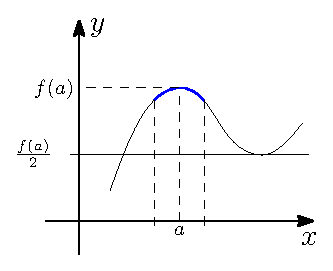
\includegraphics[width=0.3\textwidth]{17_1.eps}
			\caption{ $f(x) \geq \frac{f(a)}{2} > 0$.}
			\label{17_1}
		\end{figure}
	\end{enumerate}
\end{proof}

\newpage

\section*{Разрывность функций}

\begin{defn}
	Функция $f \colon D \to \mathbb{R}$ разрывна в точке $a$, если $f$ не является непрерывной в точке $a$.
\end{defn}

\begin{rem}
	Если $f$ разрывна в точке $a$, то $a$ - предельная точка $D$. 
\end{rem}

Функция $f$ разрывна в точке $a \Leftrightarrow \lim\limits_{x \to a} f(x)$ или не существует или существует, но $\neq f(a)$.

\begin{defn}
	Функция $f$ \uwave{разрывна в точке} $a \Leftrightarrow \nexists \lim\limits_{x \to a} f(x) \vee \exists \lim\limits_{x \to a} f(x) \neq f(a)$.
\end{defn}

\begin{defn}
	Если в точке разрыва $a, \, \exists \lim\limits_{x \to a} f(x) \neq f(a)$, то такую точку называют \uwave{точкой устранимого разрыва}.
\end{defn}

\begin{figure}[H]
	\begin{subfigure}[b]{0.5\textwidth}
		\centering
		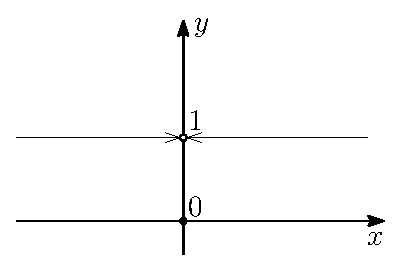
\includegraphics[width=0.6\textwidth]{17_2.eps}
		\caption{Пример точки устранимого разрыва.}
		\label{17_2}
	\end{subfigure}%
	\begin{subfigure}[b]{0.5\textwidth}
		\centering
		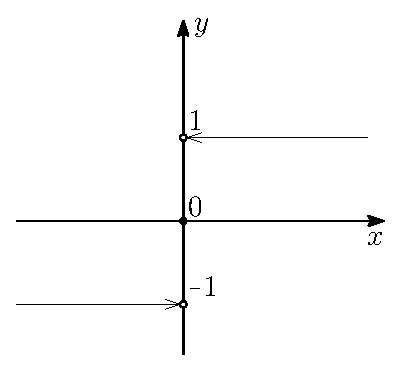
\includegraphics[width=0.55\textwidth]{17_3.eps}
		\caption{Пример точки разрыва $\RN{1}$-го рода.}
		\label{17_3}
	\end{subfigure}
\caption{Примеры точек разрыва.}
\end{figure}

\begin{defn}
	Пусть $a$ - предельная точка $D^- = (-\infty, a) \cap D$ и $D^+ = (a, +\infty) \cap D$.
	Если $\exists$ конечные пределы $\lim\limits_{x \to a-0}f(x) \wedge \! \lim\limits_{x \to a+0}f(x)$, но они различны, то говорят, что $a$ - \uwave{точка разрыва $\RN{1}$-го рода}.
\end{defn}

\begin{rem}
	Точки разрыва  $\RN{1}$-го рода - неустранимые.
\end{rem}

\begin{defn}
	Если хотя бы одного из односторонних пределов не существует (или этот предел $= \pm \infty$), то $a$ называется \uwave{точкой разрыва $\RN{2}$-го рода}.
\end{defn}

\begin{figure}[H]
	\begin{subfigure}[b]{0.5\textwidth}
		\centering
		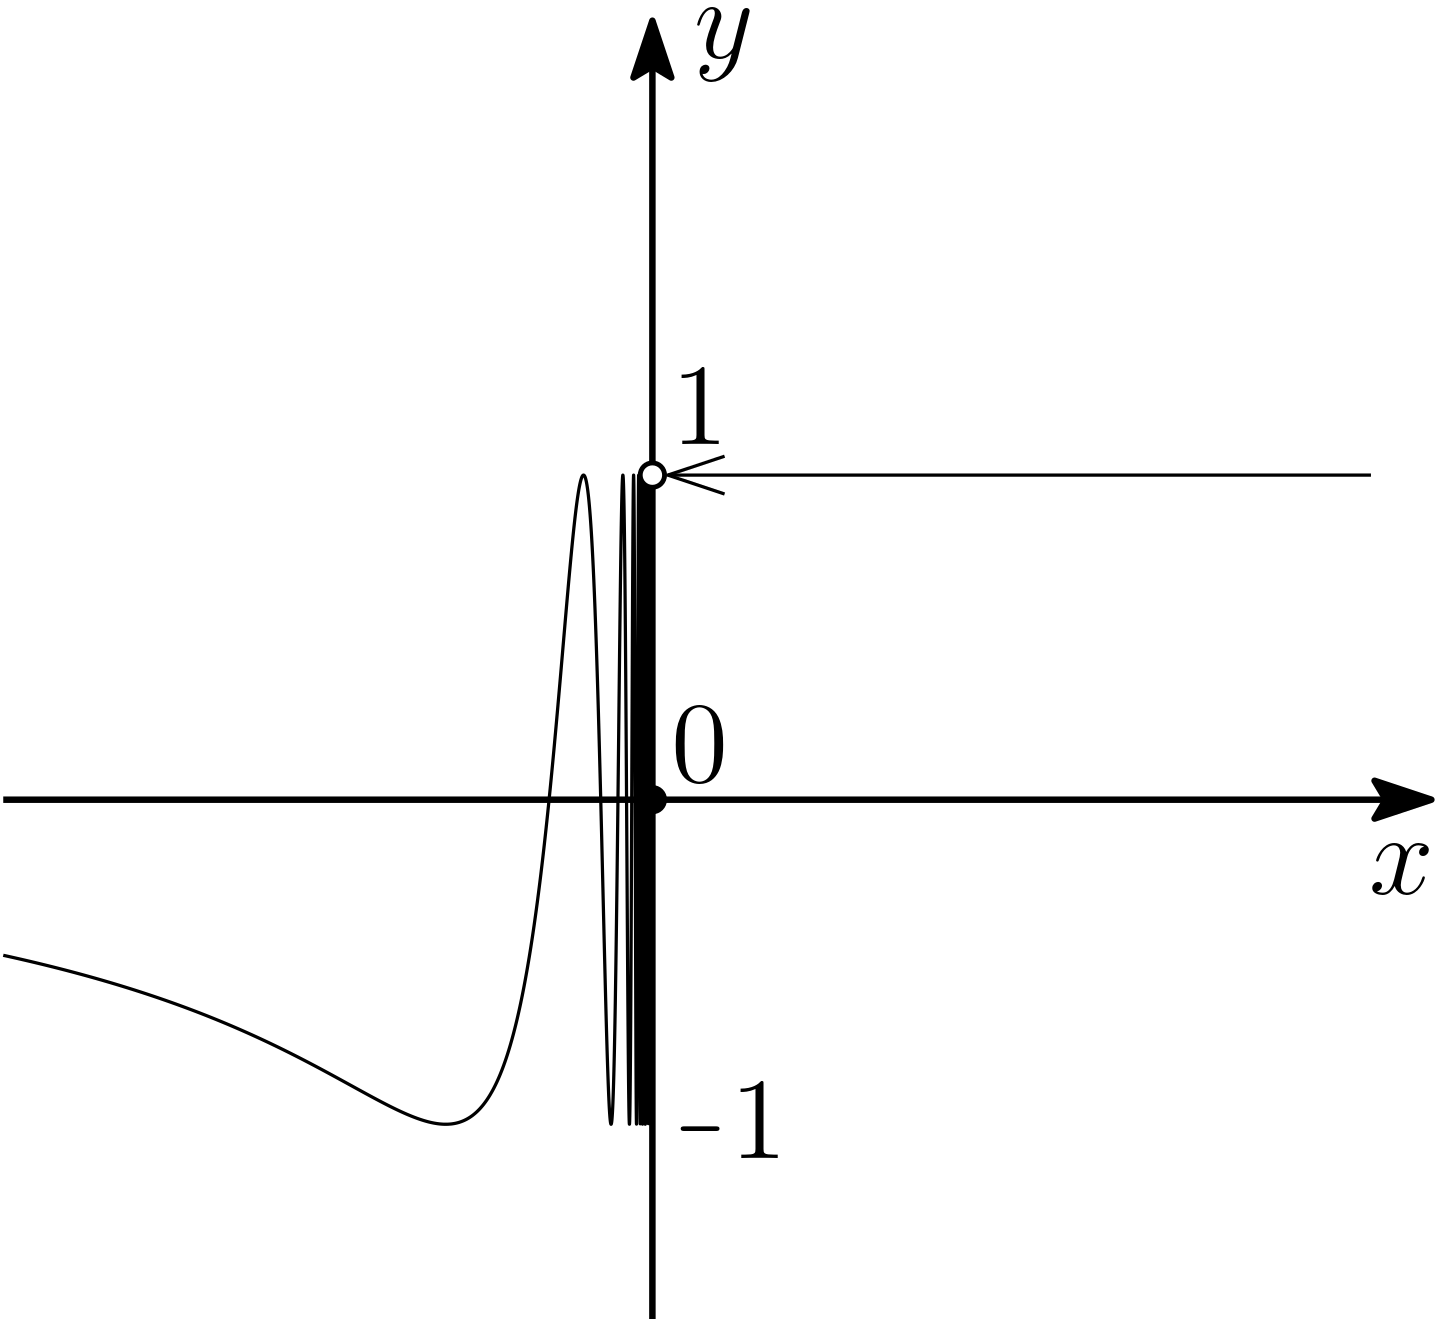
\includegraphics[width=0.6\textwidth]{17_4.png}
		\caption{$\sin{\frac{1}{x}}, \, x < 0; \, 0,\, x = 0;\, 1, \, x > 0$.}
		\label{17_4}
	\end{subfigure}%
	\begin{subfigure}[b]{0.5\textwidth}
		\centering
		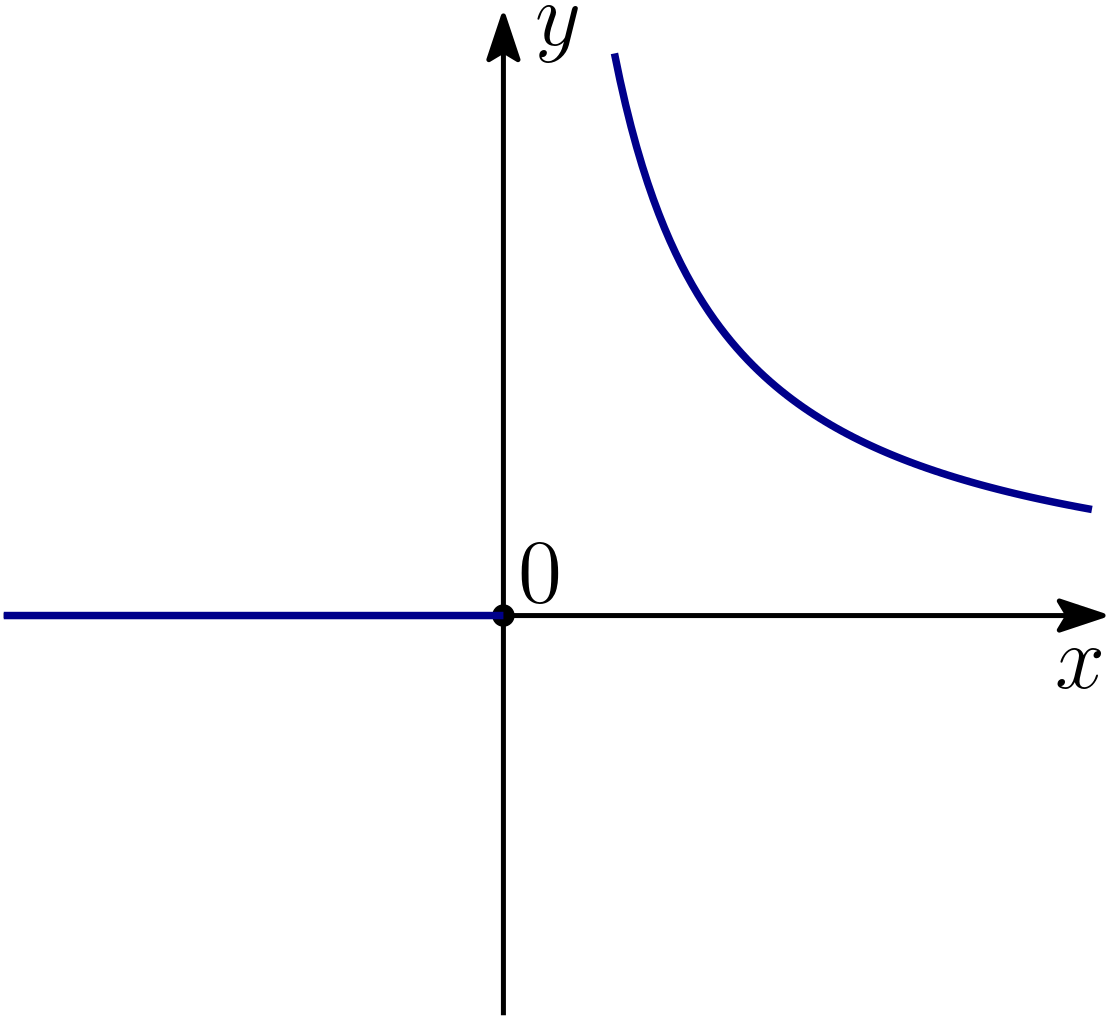
\includegraphics[width=0.55\textwidth]{17_5.png}
		\caption{$0, \, x \leq 0; \, \frac{1}{x}, \, x > 0$.}
		\label{17_5}
	\end{subfigure}
	\caption{Пример точек разрыва $\RN{2}$-го рода.}
\end{figure}


\begin{theorem}
	Пусть $f$ - определена на интервале $(\alpha, \beta)$ и монотонна. Тогда у $f$ могут быть разрывы только $\RN{1}$-го рода и множество точек разрыва не более, чем счетно.
\end{theorem}

\begin{proof}
Пусть функция $f$ не убывает. Пусть $a \in (\alpha,\beta)$. По теореме Вейрштрасса $\exists \! \! \lim\limits_{x \to a-0}f(x) = \sup\limits_{x<a}{f} = A$ и $\exists \! \! \lim\limits_{x \to a+0}f(x) = \inf\limits_{x>a}{f} = B$. Из-за монотонности $A \leq f(a) \leq B$.

\begin{figure}[H]
	\centering
	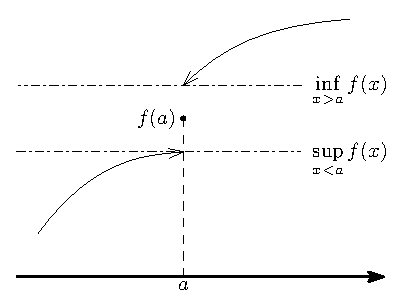
\includegraphics[width=0.4\textwidth]{17_6.eps}
	\caption{ $\sup\limits_{x<a}{f} = A \leq f(a) \leq B = \inf\limits_{x>a}{f}$.}
	\label{17_6}
\end{figure}

Если $A = f(a) = B$, то $f$ - непрерывна в точке $a$. Если $a$ - точка разрыва, то $A < f(a) \vee f(a) < B$, в частности $A \neq B$ и как следствие $a$ - точка разрыва  $\RN{1}$-го рода. 

Сопоставим каждой точке разрыва $a \mapsto (A,B)$ - непустой интервал. Пусть $a < c$ - точки разрыва и $(A,B), \, (C,D)$ - соответствующие им интервалы.

\begin{figure}[H]
	\centering
	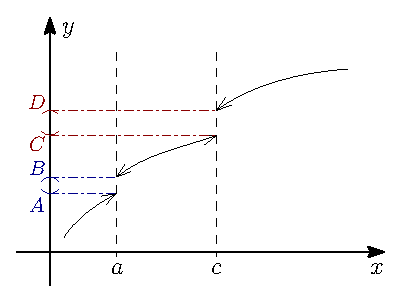
\includegraphics[width=0.4\textwidth]{17_7.eps}
	\caption{ Интервалы точек разрыва.}
	\label{17_7}
\end{figure}

Пусть $x_0 \colon a < x_0 < c \Rightarrow B \leq f(x_0) \leq C$ по определению $B$ и $C$, значит $(A,B) \cap (C,D) = \varnothing$. Таким образом, разным точкам разрывы сопоставляются разные непересекающиеся интервалы. Так как на прямой можно расположить не более чем счетный набор попарно не пересекающихся интервалов, то точек разрыва - не более чем счетно.
\end{proof}

\subsection*{Важные примеры}
\begin{enumerate}[label={\arabic*)}]
	\item \uline{Функция Дирихле}:
	$$ D(x) = \begin{cases} 
		1, & x \in \mathbb{Q} \\
		0, & x \notin \mathbb{Q} 
	\end{cases}$$
	эта функция всюду разрывна.
	\item \uline{Функция Римана}: 
		$$ R(x) = \begin{cases} 
		\frac{1}{n}, & x= \frac{m}{n} \text{ - нескоратимая дробь}\\
		0, & x \notin \mathbb{Q}\\
		1, & x = 0 
	\end{cases}$$
	эта функция разрывна в рациональных точках. Но она непрерывна в иррациональных точках.
\end{enumerate}

Можно ли придумать функцию, которая была бы разрывна во всех иррациональных точках и только в них?

\subsection*{Структура множества точек разрыва}

\begin{defn}
	Пусть $f \colon \mathbb{R} \to \mathbb{R}$ - ограниченна и $E \subset \mathbb{R}$, функция $\omega(f,E) = \sup\limits_{x,y \smallin E}|f(x) - f(y)|$ называется \uwave{колебанием функции} $f$ на множестве $E$.
\end{defn}

Пусть $f \colon \mathbb{R} \to \mathbb{R}$ - ограниченна.

\begin{prop}
	$\omega(f,E) = \sup\limits_{E}{f} - \inf\limits_{E}{f}$.
\end{prop}
\begin{figure}[H]
	\centering
	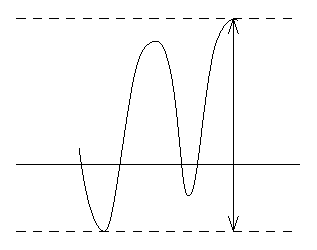
\includegraphics[width=0.25\textwidth]{17_8.eps}
	\caption{Колебание функции.}
	\label{17_8}
\end{figure}

\begin{proof}
	$f(x) - f(y) \leq \sup\limits_{E}{f} - \inf\limits_{E}{f}, \, \forall x,y \in E \Rightarrow f(y) - f(x) \leq \sup\limits_{E}{f} - \inf\limits_{E}{f}, \, \forall x,y \in E \Rightarrow$ 
	$$|f(x) - f(y)| \leq \sup\limits_{E}{f} - \inf\limits_{E}{f}, \, \forall x,y \in E \Rightarrow \omega(f,E) \leq \sup\limits_{E}{f} - \inf\limits_{E}{f}$$
	
	Пусть $\varepsilon > 0 \Rightarrow$ по определению $\exists \, x \colon \sup\limits_{E}{f} - \varepsilon < f(x)$. С другой стороны $\exists \, y \colon \inf\limits_{E}{f} + \varepsilon > f(y) \Rightarrow \sup\limits_{E}{f} - \varepsilon - (\inf\limits_{E}{f} + \varepsilon) = \sup\limits_{E}{f} - \inf\limits_{E}{f} - 2\varepsilon < f(x) - f(y) \leq \omega(f,E) \Rightarrow$
	$\forall \varepsilon >0, \, \sup\limits_{E}{f} - \inf\limits_{E}{f} < 2\varepsilon +   \omega(f,E)$. Устремим $\varepsilon \to 0$, по правилу перехода к пределу неравенства получим $\sup\limits_{E}{f} - \inf\limits_{E}{f} \leq \omega(f,E)$.
\end{proof}

Пусть $a \in \mathbb{R}$  и рассмотрим функцию $\delta \mapsto \omega(f,\mathcal{U}_\delta(a)), \, \delta >0$. Эта функция не убывает: Чем больше $\delta \Rightarrow$ тем больше окрестность $\Rightarrow$ точная верхняя грань может только возрастать. Если $\delta$ уменьшать, то к нулю эта функция будет лишь не возрастать.

\begin{figure}[H]
	\centering
	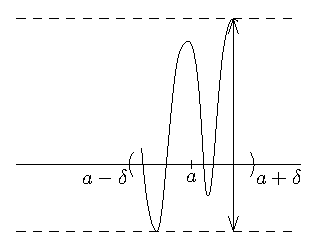
\includegraphics[width=0.25\textwidth]{17_9.eps}
	\caption{$\delta \mapsto \omega(f,\mathcal{U}_\delta(a)), \, \delta >0$.}
	\label{17_9}
\end{figure}

Снизу эта функция ограниченна: $\omega(f,\mathcal{U}_\delta(a)) \geq 0 \Rightarrow$ для не убывающей, ограниченной снизу функции мы знаем, что $\exists \! \lim\limits_{\delta \to 0+} \omega(f,\mathcal{U}_\delta(a))$. Обозначаем этот предел $\omega(f,a)$ и называем колебанием $f$ в точке $a$.
\begin{defn}
	Предел $\lim\limits_{\delta \to 0+} \omega(f,\mathcal{U}_\delta(a)) = \omega(f,a)$ называется \uwave{колебанием в точке} $a$.
\end{defn}

\begin{prop}
	$f$ непрерывна в точке $a \Leftrightarrow \omega(f,a) = 0$.
\end{prop}

\begin{proof}\hfill\\
	$(\Rightarrow)$ Пусть $f$ - непрерывна в точке $a \Rightarrow \forall \varepsilon > 0, \, \exists \, \mathcal{U}_\delta(a) \colon \forall x \in \mathcal{U}_\delta(a) \Rightarrow |f(x) - f(a)| < \varepsilon \Rightarrow \omega(f,\mathcal{U}_\delta(a)) \leq 2\varepsilon$\\
	$\Rightarrow$ при устремлении $\delta \to 0+$ такие выражения монотонно убывают $\Rightarrow \omega(f,a) \leq \omega(f,\mathcal{U}_\delta(a)) \leq 2\varepsilon$, а так как $\varepsilon$ - любое, то $\omega(f,a) = 0$.
	
	Формальнее: $\omega(f,\mathcal{U}_\delta(a)) \leq  2\varepsilon \Rightarrow \hat{\varepsilon} = \frac{\varepsilon}{2} \Rightarrow \exists \, \hat{\delta} > 0\colon \omega(f,\mathcal{U}_{\hat{\delta}}(a)) \leq 2\hat{\varepsilon} =  \varepsilon \wedge \omega(f,a) \leq \omega(f,\mathcal{U}_{\hat{\delta}}(a)) \leq \varepsilon$. И так как $\varepsilon$ - любое, то $\omega(f,a) = 0$.
	
	$(\Leftarrow)$ Пусть $\omega(f,a) = 0$ - это означает, что $\lim\limits_{\delta \to 0+} \omega(f,\mathcal{U}_\delta(a))= 0$. Знаем, что $\omega(f,\mathcal{U}_\delta(a))$ - монотонно убывает, при $\delta \to 0+ \Rightarrow \forall \varepsilon >0, \, \exists \, \delta > 0 \colon \omega(f,\mathcal{U}_\delta(a)) < \varepsilon \Rightarrow |f(x) - f(a)| < \varepsilon, \, \forall x \in \mathcal{U}_\delta(a)$.
\end{proof}

\begin{corollary}
	Множество точек разрыва $ = \bigcup\limits_{n}\{\,a \colon \omega(f,a) \geq \frac{1}{n} \,\}$.
\end{corollary}

\begin{prop}
	Множество $\bigcup\limits_{n}\{\,a \colon \omega(f,a) \geq \frac{1}{n} \,\}$ - замкнуто.
\end{prop}

Таким образом, множество точек разрывов это не более чем счетное объединение замкнутых множеств.
\end{document}